\documentclass[12pt, ams, nofootinbib]{revtex4}
%\documentclass[12pt,preprint,ams, nofootinbib]{revtex4-1}
%\documentclass{revtex4-1}
\usepackage{amsmath}
\usepackage{amsfonts}
\usepackage{amsthm}
\usepackage{amssymb}
\usepackage{graphicx}  %for \scalebox	
\usepackage{mathtools} %for \dcases
\usepackage{epsfig}
\usepackage[colorlinks=true,urlcolor=blue,linkcolor=blue]{hyperref}
\usepackage{amscd}
%\usepackage[color,draft]{showkeys}
\usepackage{xcolor}
%\usepackage{enumitem}
\usepackage{enumerate}
\usepackage{frcursive}
\usepackage[T1]{fontenc}
\usepackage[toc]{appendix}
%\usepackage[bottom]{footmisc}
\usepackage{mathrsfs}
\usepackage{tensor}     % index positioning in tensor componentes: \tensor{M}{^a_b^c_d}
\usepackage{multirow}

%% Commands
\newtheorem{theorem}{Theorem}%[section]
\newtheorem{corollary}{Corollary}%[section]
\newtheorem{lemma}{Lemma}%[section]

%% Definitions
% Comands
\def\be{\begin{equation}}
\def\ee{\end{equation}}
\def\bpr{\begin{proof}}
\def\epr{\end{proof}}

% Functions
\def\arcsinh{{\rm arcsinh}}
\def\sign{{\rm sign}}
\def\min{{\rm min}}

% Expressions
\def\X{\Lambda}
\def\Y{\Upsilon}
%\def\e{\text{e}}
\def\e{e}
\def\A{\mathcal{A}}
\def\B{\mathcal{B}}
\def\ehat{\hat{\text{\textbf{\textit{e}}}}}
\def\ihat{\hat{\boldsymbol{\imath}}}
\def\jhat{\hat{\boldsymbol{\jmath}}}
\def\khat{\hat{\text{\textbf{\textit{k}}}}}
\def\bnabla{\boldsymbol{\nabla}}
\def\Sinh{{\rm sinh}}  %To avoid the small space between the function and the argument
\def\Cosh{{\rm cosh}}


%% New commands
\newcommand{\rob}[1]{\left(#1\right)}    % Round brackets
\newcommand{\sqb}[1]{\left[#1\right]}    % Square brackets
\newcommand{\mb}[1]{\mathbf{#1}}         % Math bold face
\newcommand{\cub}[1]{\left\{#1\right\}}  % Curly brackets
\newcommand{\abb}[1]{\left|#1\right|}    % Absolute value brackets
\newcommand{\mbi}[1]{\boldsymbol{#1}}    % Math bold and math italic face 
\newcommand{\mc}[1]{\mathcal{#1}}        % \mathcal
\renewcommand{\Re}{\mathbb{R}}           % Real numbers
\newcommand{\ba}[1]{\begin{align}#1 \end{align}}          % Align
\newcommand{\partd}[2]{\frac{\partial #1}{\partial #2}}   % Partial derivative
\newcommand\scalemath[2]{\scalebox{#1}{\mbox{\ensuremath{\displaystyle #2}}}}

%% Theorem commands
\theoremstyle{definition}
\newtheorem{defn}{Definition}[section]
\newtheorem{conj}{Conjecture}[section]
\newtheorem{exmp}{Example}[section]
\newtheorem{prop}{Proposition}[section]
%\theoremstyle{Identity}
%\newtheorem{identity}{Identity}[section]

\begin{document}

\preprint{APS/123-QED}
%\title{The Ovoid Coordinate System}
%\title{Ovoid coordinates for applications in astrophysics}
%\title{New systems of orthogonal curvilinear coordinates to describe ovoid spacetimes}
%\title{New sets of orthogonal coordinates that generalize conic coordinates to describe ovoid spacetimes}
%\title{New orthogonal systems of coordinates, based on a generalization of conics, to construct ovoid spacetimes}
%\title{New orthogonal systems of coordinates based on Cartesian ovals to construct ovoid spacetimes}
%\title{A new orthogonal ovoid coordinate system to describe ovoid spacetimes}
%\title{Some new ovoid coordinate systems to describe ovoid spacetimes}
%\title{New ovoid coordinate systems and their application to construct ovoid spacetimes}
%\title{New ovoid coordinate systems and new ovoid spacetimes}
%\title{Construction of ovoid coordinate systems and ovoid spacetimes}
%\title{Construction of new ovoid coordinate systems to describe ovoid spacetimes}

\title{Construction of ovoid coordinate systems and ovoid spacetimes}
%\title{Construction of ovoid coordinate systems to describe ovoid spacetimes}

\author{Juan A. Guarín-Rojas}
\email{juan2201870@correo.uis.edu.co}
\affiliation{Escuela de Física, Universidad Industrial de Santander, CP 680002,  Bucaramanga, Colombia.}

\author{Antonio C. Guti\'errez-Pi\~{n}eres}
\email{acgutier@uis.edu.co}
\affiliation{Escuela de Física, Universidad Industrial de Santander, CP 680002,  Bucaramanga, Colombia}
\affiliation{Instituto de Ciencias Nucleares, Universidad Nacional Aut\'onoma de M\'exico,
 AP 70543,  M\'exico, CDMX 04510, M\'exico}

\author{Rafael Torres}
\email{rafael.torres@saber.uis.edu.co}
\affiliation{Escuela de Física, Universidad Industrial de Santander, CP 680002,  Bucaramanga, Colombia}

\date{\today}


%%%%%%%%%%%%%%%%%%%%%%%%%%%%%%%%%%%%%%%%%%%%%%%%%%%%%%%%%%
%%%%%%%%%%%%%%%%%%%%%%%%%%%%%%%%%%%%%%%%%%%%%%%%%%%%%%%%%%
\begin{abstract} 
In this work, some Cartesian ovoid coordinates are constructed to facilitate the description of ovoid spacetimes. In optics, Cartesian ovoids are very useful for constructing optical systems without both geometric and chromatic aberrations. In astrophysics, these ovoids may be useful for describing objects with mass quadrupoles, such as merging binary stars. Then, ovoid spacetimes could be of interest to the scientific community. To construct ovoid coordinates, two special families of ovals are considered: confocal and triconfocal ovals. In the first family, the ovals share two foci, and in the second one, they share three. For both cases, another family of curves is found such that any of its members intersects the curves of its respective family of ovals at right angles. Then, some 2D coordinates are inferred from these families of curves. These coordinates are extended to 3D, yielding cylindrical and rotational-like coordinates. From the Euclidean line element in ovoid coordinates, a metric ansatz for describing a stationary ovoid spacetime is proposed. Next, this ansatz is used to obtain an exact solution of the Einstein field equations for a static anisotropic fluid.
\end{abstract}

%Remark: Pascal limaçon have not been reported before in the literature.

%\pacs{}

\maketitle

%%%%%%%%%%%%%%%%%%%%%%%%%%%%%%%%%%%%%%%%%%%%%%%%%%%%%%%%%%
%%%%%%%%%%%%%%%%%%%%%%%%%%%%%%%%%%%%%%%%%%%%%%%%%%%%%%%%%%
\section{Introduction} %Mencionar: *óvalos en la óptica, *aplicación en astrofísica
\label{sec:intro}
Cartesian ovoids are quartic surfaces that have been proven to be useful in optics. They were found as a solution to the problem of rigorous stigmatism \cite{silva-Lora2020a}, in which light rays emitted from a point source must be refracted to a single point by an optical surface, which turns out to be a Cartesian ovoid \cite{descartes1637, southall1922}. In a plane containing the focal axis, one obtains a Cartesian oval as the intersection curve between the ovoid and the plane. In recent years, Cartesian ovoids have been recovered by Silva-Lora and Torres \cite{silva-Lora2020c, silva-Lora2021, silva-Lora2022}. These authors use ovoids to construct singlet lenses with aplanatism and compound lenses with achromatic stigmatism, i.e., stigmatic systems free of chromatic aberration. These promising results show the importance of ovoids in optics.

Ovoids can also be considered as a specialization of the family of superconic surfaces	 \cite{Greynolds2002, Cho2016, silva-Lora2020b}. These surfaces satisfy an algebraic equation of $n$th degree that generalizes the Schwarzschild equation for conic surfaces\footnote{Hereafter, conic surfaces refer to the surfaces of revolution of conic sections.} \cite{schwarzschild1905conic, silva-Lora2020b}. They have been proposed for use in optical design. Ovoids are also close to conic surfaces in that their respective curves, ovals and conic sections, both have foci. However, ovals have three foci \cite{chasles1837, williamson1873, johnson1875bipolar}. When one of the foci goes to infinity, the Cartesian ovals become conic sections \cite{chasles1837, johnson1875bipolar}, or a portion of them, and when the third focus coincides with the first or the second, they become limaçons of Pascal \cite{johnson1875bipolar}. In this way, ovoids generalize conic surfaces. 
%\footnote{See note XXI of \cite{chasles1837} and chapter XX of \cite{williamson1873}.}

In general relativity, symmetries are key to simplifying the description of spacetimes. The most common symmetries used to model astrophysical objects are spherical and axial symmetry. Models with these symmetries are widely found in the literature \cite{schwarzschild1916fluid,tolman1939static,wahlquist1968interior,chinea1990interior}. Within axially symmetric spacetimes, there are the ellipsoidal spacetimes formulated by Krasiński \cite{Krasinski1978}. Some authors have found solutions to the Einstein field equations based on Krasiński's work, recovering known solutions and obtaining new ones \cite{Racz1992,racz1998uniqueness, Zsigrai2003}. Hence, spherical and ellipsoidal symmetry have been useful to construct spacetimes in general relativity.

Since spheres and ellipsoids are special cases of Cartesian ovoids, one wonders if ovoids can also be useful to construct spacetimes in general relativity. As ovoids resemble deformed spheres, one would expect that an astrophysical object with this shape must have a mass quadrupole. This quadrupole would allow the object to emit gravitational waves in a perturbative regime \cite{misner2017gravitation}. Then, ovoids might be useful to describe the gravitational waves emitted by binary neutron stars during merger. As the stars coalesce, they get deformed and form some kind of funnel that could be modeled using an ovoid.

The purpose of this work is to construct some ovoid spacetimes as candidates to model the gravitational field of an ovoid-shaped object. To that end, Sections \ref{sec:Cartesian ovals}-\ref{sec:characterization} introduce Cartesian ovals and ovoid coordinates. In Section \ref{sec:Cartesian ovals}, Cartesian ovals are treated as a three-foci curve, and their existence condition is shown. Section \ref{sec:families of ovals} presents confocal and triconfocal ovals and their respective orthogonal curves. Based on the curves discussed above, Section \ref{sec:characterization} formulates and characterizes ovoid coordinates. The transformation rules between ovoid and Cartesian coordinates, and the line elements in the new coordinates are obtained.

In general relativity, symmetry can be described in terms of isometry groups and geometric invariants such as Killing vectors \cite{StephaniKramer2003}. This description applies to spherical, axial, and time-translation symmetries. To extend the notion of symmetry, Krasiński's pioneering work \cite{Krasinski1978} defines ellipsoidal spacetimes in terms of a congruence of observers and the induced metric. Whether isometries or Killing vectors can characterize these spacetimes remains an open question. For now, this work focuses on proposing a metric ansatz rather than characterizing its symmetry. Based on Krasiński's ideas, Section \ref{sec:ovoid spacetimes} defines ovoid spacetimes using the induced metric on confocal ovoids. In Section \ref{sec:solutions}, exact solutions to the Einstein field equations for a static anisotropic fluid in an ovoid spacetime are obtained.


\section{Cartesian ovals} %Mencionar: *Cond. de existencia, *Ecs. bipolares (3er foco)
\label{sec:Cartesian ovals}
A Cartesian oval is the locus of points $M$ such that $cr+cr’$ is constant, where $r$ and $r’$ are the distances from $M$ to two fixed points $F$ and $F’$, called foci, and $c$ and $c’$ are real constants \cite{williamson1873, johnson1875bipolar}. Since $c$ and $c’$ cannot both be zero, one can assume $c\neq 0$ without loss of generality. Hence, the equation satisfied by Cartesian ovals can be written as
\be 
	r+ar' = u\,, \label{eq:oval}
\ee
where $a$ and $u$ are real constants. 

For any oval with known foci $F$ and $F'$, there exists a third point $F''$ such that the oval satisfies an analog of equation \ref{eq:oval} of the form $r+\alpha r''=\beta$, where $r$ and $r''$ are the distances from $M$ to $F$ and $F''$, and $\alpha$ and $\beta$ are real constants. This point lies on the line through $F$ and $F'$ and is called the third focus. 

The existence of this point was first noted by Chasles; see Note XXI in \cite{chasles1837}. In \cite{chasles1837, williamson1873}, geometric constructions are used to obtain the third focus. Here, an algebraic approach that recovers the results of \cite{johnson1875bipolar} is presented.

To determine the position of the third focus, consider an $xy$-coordinate system centered at $F$ with $F'$ at $(\tau,0)$, as shown in Fig. \ref{fig:oval}. Allow $\tau$ to be either positive or negative. In this coordinate system, equation \ref{eq:oval} can be written as 
\be
	\sqrt{x^2+y^2}+a \sqrt{(x-\tau)^2+y^2}=u\,. \label{eq:oval xy-cord}
\ee
In polar coordinates, related to $x$ and $y$ by $x=r\cos\theta$ and $y=r\sin\theta$, this equation becomes $r+\sqrt{r^2-2r\tau\cos\theta+\tau^2}=u$. Consider that $F''$ is located at $(\tau+\xi,0)$ where $\xi\in\Re$. By definition, the distance from $M$ to $F''$ is
\begin{align}
	r'' &= \sqrt{(x-\tau-\xi)^2+y^2}\,, \\
		&= \sqrt{r^2-2r(\tau+\xi)\cos\theta+(\tau+\xi)^2}\,.
\end{align}
From the last equation, one obtains $-2r\tau\cos\theta=\tau(r''^2-r^2-(\tau+\xi)^2)/(\tau+\xi)$. Hence, equation \ref{eq:oval xy-cord} in polar coordinates becomes
\be
	r+\sqrt{r^2+\frac{\tau}{\tau+\xi}(r''^2-r^2-(\tau+\xi)^2)+\tau^2}=u\,.
\ee
This equation can be solved for $r''^2$, yielding
\be
	r''^2 = \frac{(u-r)^2(\tau+\xi)}{a^2\tau}+(\tau+\xi)\xi -\frac{r^2\xi}{\tau}\,.
\ee
Now, one can group the terms in $r$ and complete the square on the right-hand side of the equation as
\be
	r''^2=\frac{1}{a^2\tau}\left(\tau+(1-a^2)\xi\right)\left(r-\frac{u(\tau+\xi)}{\tau+(1-a^2)\xi}\right)^2 + \frac{\xi(\xi+\tau)}{\xi+\tau/(1-a^2)}\left(\xi-\frac{u^2-\tau^2}{(1-a^2)\tau}\right)\,. \label{eq:def xi}
\ee
%\be
%	r''^2=\frac{\tau+\xi}{a^2\tau}\left(1-\frac{a^2\xi}{\tau+\xi}\right)\left(r-\frac{u(\tau+\xi)}{\tau+(1-a^2)\xi}\right)^2 + \frac{\xi(\xi+\tau)}{\xi+\tau/(1-a^2)}\left(\xi-\frac{u^2-\tau^2}{(1-a^2)\tau}\right)\,. \label{eq:def xi}
%\ee
The second term is zero when $\xi=0$, $\xi=-\tau$, and $\xi=\frac{u^2-\tau^2}{(1-a^2)\tau}$. For these values of $\xi$, the relation between $r''$ and $r$ is linear. Replacing $\xi$ with $0$, $-\tau$, and $\frac{u^2-\tau^2}{(1-a^2)\tau}$, equation \ref{eq:def xi} becomes, respectively,
\be
	r''^2 = \frac{(u-r)^2}{a^2}\,,
\ee
\be
	r''^2 = r^2\,,
\ee
\be
	r''^2 = \frac{u^2}{a^2\tau^2}\rob{r-\frac{u^2-a^2\tau^2}{u(1-a^2)}}^2\,. \label{eq:oval^2 third_focus}
\ee
Thus, the known cases are recovered, and one new result is obtained. The first case, $\xi=0$, corresponds to $F''$ coinciding with $F'$, while the second, $\xi=-\tau$, corresponds to $F''$ coinciding with $F$. The third case is the only genuinely new result. In this case, $F''$ is located at $(\frac{u^2-a^2\tau^2}{(1-a^2)\tau},0)$. By convention, the expression for $\xi$ is henceforth fixed as
\be
	\xi = \frac{u^2-\tau^2}{(1-a^2)\tau}\,. \label{eq:def xi}
\ee

From equation \ref{eq:oval^2 third_focus}, it follows an equation of the form $r''=\pm c_1(r-c_2)$, where $c_1$ and $c_2$ are constants. The $\pm$ sign must be replaced with the sign of $\tau(1-a^2)$ so that the resulting curve coincides with the curve defined by equation \ref{eq:oval}, as one can verify in plotting software. The resulting linear equation in $r$ and $r''$ is therefore
\be
	\sign(\tau(1-a^2)) ar''+\frac{u}{\tau}r=(\tau+\xi)\,,\label{eq:oval bipolar2}
\ee
where $\sign(x):=x/|x|$ is the sign function and $\xi$ is given by equation \ref{eq:def xi}. Substituting $r$ from \ref{eq:oval}, this equation becomes
\be 
	\sign(\tau(1-a^2))r''-\frac{u}{\tau}r'=a\xi\,. \label{eq:oval bipolar3}
\ee
Equations \ref{eq:oval}, \ref{eq:oval bipolar2}, and \ref{eq:oval bipolar3} are the so-called bipolar equations of the Cartesian oval \cite{johnson1875bipolar}.

The procedure for finding $F''$ just shown here has not been presented in this form elsewhere. However, the equations presented here are equivalent to those in \cite{johnson1875bipolar}. The authors considered it a good idea to revisit Johnson's work using modern, clean notation.

%To end this section, consider the next question: given the points $F$ and $F'$, for which values of $a$ and $u$ the curve defined by equation \ref{eq:oval} is not empty. As it turns out, $a$ and $u$ must satisfy $u\geq \min(1,a)|\tau|$ if $a>-1$, $u\leq|\tau|$ if $a<-1$ and $-|\tau|\leq u\leq |\tau|$ if $a=-1$, where $\min(x, y)$ is defined as the minimum value between $x$ and $y$. These are the \textit{existence conditions} for Cartesian ovals.

In \cite{quelet1829}, Quelet first observed that Cartesian ovals can be obtained by intersecting two cones with parallel axes. From equation \ref{eq:oval xy-cord}, it is easy to see that Cartesian ovals can be obtained by intersecting the cones defined by the equations
\be
	z=\sqrt{x^2+y^2}\,,
\ee
\be
	z=u-a\sqrt{(x-\tau)^2+y^2}\,.
\ee
Let the first be called the fixed cone (FC) and the second the movable cone (MC). The values of $u$, $a$, and $\tau$ control the location of the apex and the apex angle of the MC. For some values of these constants, the two cones may not intersect. In such cases, one says that the curve is empty, i.e., that no point satisfies equation \ref{eq:oval}.

Hence, by analyzing when cones intersect each other, one can obtain the \textit{existence condition} on $u$, $a$ and $\tau$ such that the curve defined by equation \ref{eq:oval xy-cord} is nonempty. This analysis can be divided into three main cases, $|a|<1$, $a>1$ and $a<-1$, and two limit cases, $a=\pm 1$. For $|a|<1$, the cones intersect if the $z$-intercept of the MC is at or above the origin, as shown in Fig. \ref{fig:cones_1_3}. This implies $u-a|\tau|\geq 0$. For $a>1$, the cones intersect if the apex of the MC is at or above the FC, as shown in Fig. \ref{fig:cones_2_4}. Thus, $u\geq |\tau|$. Conversely, for $a<-1$, the cones intersect if the apex of the MC is at or below the FC, as shown in Fig. \ref{fig:cones_2_4}. Then, one needs $u\leq|\tau|$.

In the limiting cases $a=\pm 1$, the two cones have the same apex angle of $\pi/2$. For $a=1$, the cones open in opposite directions. In this case, the apex and the $z$-intercept of the MC are both at or above the FC when $u\geq|\tau|$. This is the existence condition for $a=-1$. In the last case, $a=-1$, two conditions are required: the MC's apex must be at or below the FC, and the MC's $z$-intercept must be at or above the origin. This translates to $-|\tau|\leq u \leq |\tau|$.

The existence condition of Cartesian ovals can be summarized as follows
\be
u\geq \min(1,a)|\tau|,\qquad \text{if } a>-1;	\label{eq:cond_c1}
\ee
\be
u\leq|\tau|,                  \qquad \text{if } a<-1;	\label{eq:cond_c2}
\ee 
\be
-|\tau|\leq u\leq|\tau|,      \qquad \text{if } a=-1\,. \label{eq:cond_c3}
\ee
where $\min(x, y)$ is defined as the minimum of $x$ and $y$. As far as the authors know, the existence conditions \ref{eq:cond_c1}-\ref{eq:cond_c3} are not in the literature. Nevertheless, one can argue that they are implicit in the work of Descartes \cite{descartes1637}, and they are mentioned by R. Ferréol on his math blog \cite{mathcurve}. At the time of writing this article, the condition for $a< -1$ in \cite{mathcurve} is incorrect, but the other one is correct. %One could also argue that these conditions are implicit in the work of descartes \cite{descartes1637}.

%As an interesting final remark, the apex of the MC is a point in the intersection curve when $u=-\min(-1,-|a|)|\tau|$. For this value of $u$, the Cartesian oval is a limaçon of Pascal, or a part of it.

\begin{figure}
	\centering
	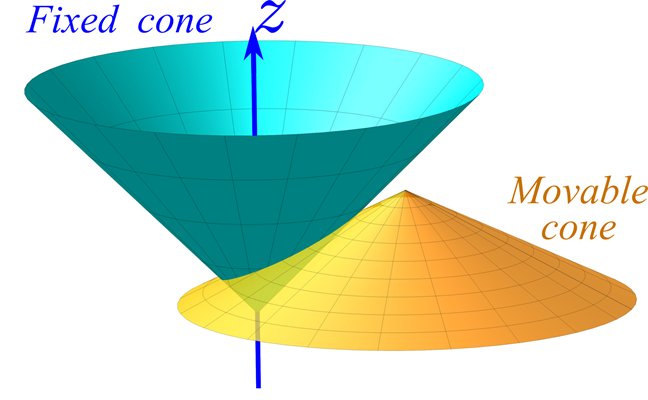
\includegraphics[width = 0.4 \textwidth]{images_low_resolution/cones1.png}
	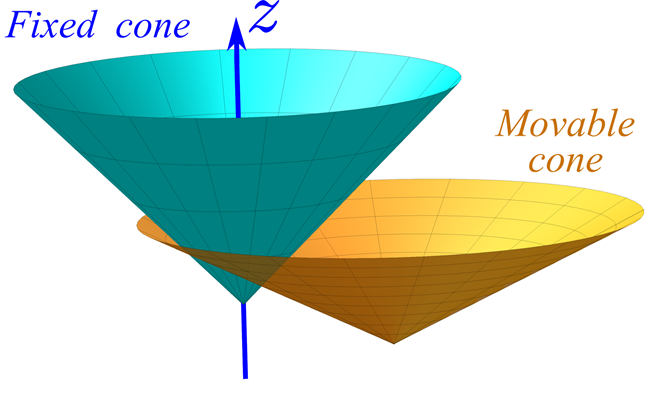
\includegraphics[width = 0.4 \textwidth]{images_low_resolution/cones3.png}
	\caption{The fixed cone (FC) and the movable cone (MC) for the cases $0<a<1$ and $-1<a<0$. On the left, $a=1/2$ and $u=0.85$; on the right, $a=-1/2$ and $u=-0.3$. In both cases, $\tau=1$. Because of the form of the cones, the intersection curve exists if the MC's $z$-intercept is at or above the origin.}
	\label{fig:cones_1_3}
\end{figure}

\begin{figure}
	\centering
	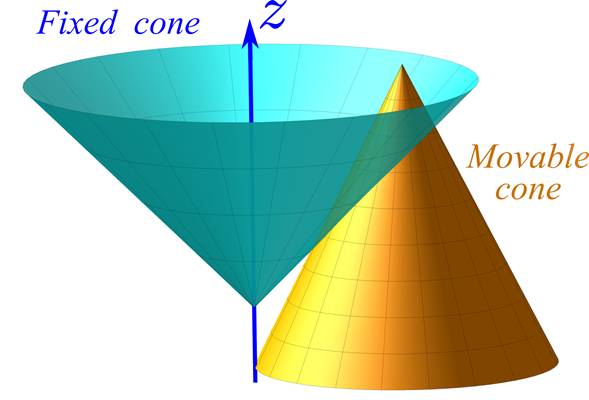
\includegraphics[width = 0.4 \textwidth]{images_low_resolution/cones2.png}		
	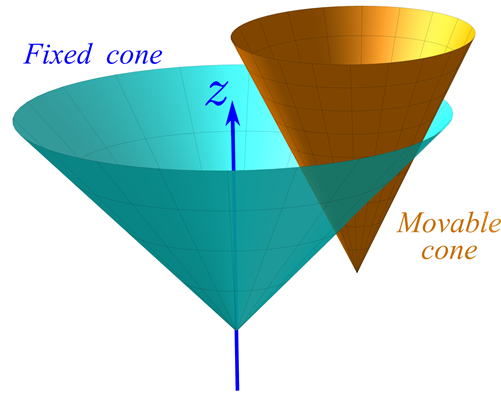
\includegraphics[width = 0.35 \textwidth]{images_low_resolution/cones4.png}
	\caption{The fixed cone (FC) and the movable cone (MC) for the cases $a>1$ and $a<-1$. On the left, $a=2$ and $u=1.6$; on the right, $a=-2$ and $u=0.5$. In both cases, $\tau=1$. The condition for the cones to intersect depends only on the MC's apex location.}
	\label{fig:cones_2_4}
\end{figure}

\section{Two remarkable families of ovals and their respective orthogonal curves}
\label{sec:families of ovals}
This section describes two families of Cartesian ovals that will be used to construct orthogonal coordinates. For each family, $\mathfrak{F}$, a second family of curves, $\mathfrak{G}$, will be obtained so that the members of $\mathfrak{F}$ intersect those of $\mathfrak{G}$ at right angles. The resulting pairs of families, such as $\mathfrak{F}$ and $\mathfrak{G}$, produce a curvilinear grid with right angles at each vertex. This allows the construction of an orthogonal coordinate system, as shown in Section \ref{sec:characterization}.

The members of each family are characterized by the value of a parameter $u_i$, so each vertex on the grid is labeled with a pair $(u_1, u_2)$. The relations between this pair of values and the $xy$-coordinates of the vertex, $(x,y)$, with respect to a given $xy$-coordinate system are derived in each subsection. These relations provide the coordinate transformations between the rectangular and the new coordinates, as will be shown in Section \ref{sec:characterization}.

\subsection{Confocal ovals and synecdolas} % *Def. sinécdolas, *Mapeo inverso [de (u,v) a (x,y)], *Mencionar caso a=1, *Hacer caso a=1/3
\label{sec:confocal}
Consider the family of level curves of the function $f$ defined by
\be
	f(x,y)=\sqrt{x^2+y^2}+a \sqrt{(x-\tau)^2+y^2}\,,
\ee
where $a$ and $\tau$ are fixed constants. These level curves are ovals with the same focal distance $|\tau|$ and the same value of $a$. Hence, they can be called \textit{confocal ovals} or, more precisely, \textit{biconfocal ovals} since they share the same two of the three foci. Here, they are referred to simply as confocal ovals. The level curves satisfy the equation $f(x,y)=u$, where $u$ is a constant. As the value of $u$ varies, the curves cover the entire $xy$-plane, as shown in Fig. \ref{fig:confocal_ovals}. The quantity $u$ may take only values that satisfy one of the existence conditions of ovals \ref{eq:cond_c1}-\ref{eq:cond_c3}, depending on the value of $a$.

\begin{figure}[h]
	\centering
	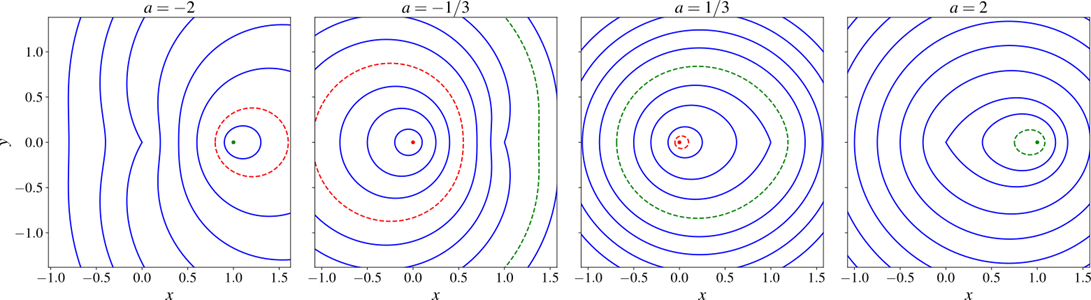
\includegraphics[width = \linewidth]{images_low_resolution/ovals.png}
	\caption{Level curves of $f$ for different values of $a$ with $\tau=1$, which correspond to confocal ovals. The subfigures show the four characteristic sets of confocal ovals for $a\in(-\infty,-1)$, $a\in(-1,0)$, $a\in(0,1)$, and $a\in(1,\infty)$, in order from left to right. All subfigures share the same $y$-axis limits. Some ovals are colored to illustrate how they change as $a$ varies; the red one corresponds to $u=0.4$, while the green one corresponds to $u=1.25$.} %In the limit cases $a=-1,0,1$, confocal ovals become branches of hyperbolas, circles, and ellipses, respectively.
	\label{fig:confocal_ovals}
\end{figure}

Consider now the problem of finding the curves orthogonal to confocal ovals. The gradient of $f$ is a vector field orthogonal to the level curves of $f$. Therefore, the orthogonal curves must have tangent vectors proportional to $\nabla f$. This condition yields
\be
	\frac{dy}{dx}=\frac{f_x}{f_y}\,, \label{eq:ODE}
\ee
where the subscripts in $f$ denote partial derivatives and the orthogonal curves are assumed to satisfy $y=y(x)$. In its differential form, the equation \ref{eq:ODE} becomes $f_ydx-f_x dy=0$, an inexact differential equation. However, it can be made exact by the integrating factor $w=1/y$, so that $(f_y/y)dx-(f_x/y) dy=0$ is exact. The implicit solution of this equation is
\be
	\arcsinh{\rob{\frac{x}{y}}} + a\, \arcsinh{\rob{\frac{x-\tau}{y}}} = v\,,
\ee
where $v$ is a real constant. Let $g$ be a function with $g(x,y)$ defined as the left-hand side of this equation. The set of level curves of $g$ will be called synecdolas. Each of these curves crosses each confocal oval at a right angle. For $a=1$, synecdolas become sections of hyperbolas, and for $a=-1$ they become the upper or lower halves of ellipses. In Figure \ref{fig:synecdolas}, some synecdolas are plotted for $a=1/3$. The term \textit{synecdola} derives from the figure of speech ``synecdoche''. The term was coined, inspired by the similarity between the names of conic sections and figures of speech, such as circle and circumlocution, ellipse and ellipsis, hyperbola and hyperbole, and parabola and parable.

\begin{figure}[h]
	\centering
	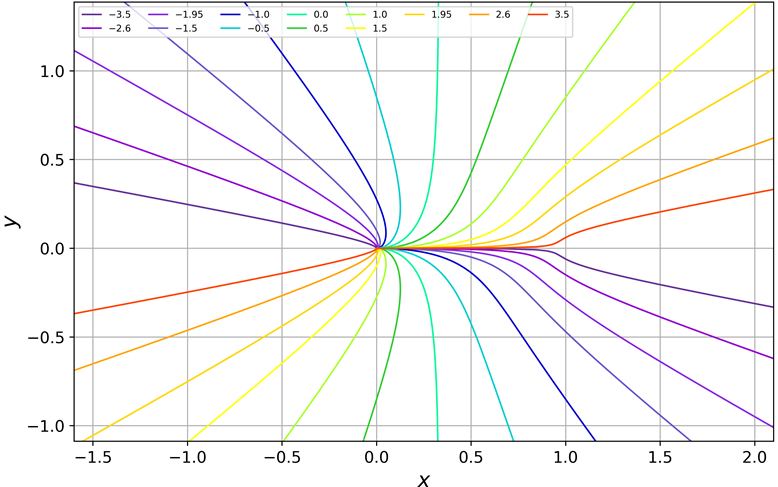
\includegraphics[width = 0.8 \textwidth]{images_low_resolution/synecdolas1.png}
	\caption{Synecdolas for $a=1/3$, $\tau=1$ and different values of $v$. These curves resemble confocal hyperbolas. Each one is composed of two branches connected at the origin that converge to a straight line at infinity.}
	\label{fig:synecdolas}
\end{figure}

Synecdolas and confocal ovals form a pair of families whose curves intersect at right angles. The inverse relations $x=x(u,v)$ and $y=y(u,v)$, obtained by solving the equations $f(x,y)=u$ and $g(x,y)=v$ for $x$ and $y$, provide the relations between Cartesian coordinates and the new coordinates $u$ and $v$. To obtain the inverse relations, consider the substitutions
\be
	x=\frac{\tau\sinh t}{\sinh t-\sinh{\rob{\frac{v-\tau}{a}}}}\,, \label{eq:x(t)}
\ee
\be
	y=\frac{\tau}{\sinh t-\sinh{\rob{\frac{v-\tau}{a}}}}\,. \label{eq:y(t)}
\ee
These are the parametric equations for the synecdola. Substituting them into $g(x,y)=v$ yields $v=v$, so the equation is automatically satisfied. The remaining equation, $f(x,y)=u$, becomes
\be
	\frac{|\tau|\rob{\cosh{t}+a\,\Cosh{\rob{\frac{v-t}{a}}}}}{\abb{\sinh t-\Sinh\rob{\frac{v-t}{a}}}} = u\,. \label{eq:general_u}
\ee
The expression in absolute value equals $|y|$, where $y$ is taken from equation \ref{eq:y(t)}. Hence, by considering inverse relations with $y=y(u,v)>0$, equation \ref{eq:general_u} becomes
\be 
	(a\tau-u)s^{\frac{2}{a}}+ \e^{\frac{v}{a}}(\tau-u)s^{\frac{1}{a}+1} + \e^{\frac{v}{a}}(\tau+u)s^{\frac{1}{a}-1}+\e^{\frac{2v}{a}}(a\tau+u) = 0\,,
\ee
where $s=\e^t$. For $a\in\mathbb{Q}$, this equation can be rearranged into an algebraic equation of a certain degree, as shown in Appendix \ref{sec:appendix-s-equation}. For $a=1/3$, it becomes a cubic in $s^2$ whose positive real solution for $s$ is
\be
	s = \sqrt{\alpha_+^{\frac{1}{3}} + \alpha_{-}^{\frac{1}{3}}-\frac{(\tau-u)\e^{3v}}{\tau-3u}}\,, \label{eq:sol_s1/3}
\ee
where
\begin{align}
	\alpha_{\pm} =& \pm \frac{\e^{\frac{9v}{2}}}{(\tau-3u)^2}\sqrt{\sqb{(\tau+3u)(\tau-u)^3\e^{3v}-(\tau-3u)(\tau+u)^3}(\e^{3v}-1)} \notag \\  
				&-\frac{\e^{6v}}{(\tau-3u)^3} \sqb{(\tau-u)^3\e^{3v}-(\tau-3u)(\tau^2+3u^2)}\,. \label{eq:sol_s1/3_aux}
\end{align}
By successively substituting $t=\ln s$ and equations \ref{eq:sol_s1/3} and \ref{eq:sol_s1/3_aux} in equations \ref{eq:x(t)} and \ref{eq:y(t)}, one obtains the desired relations $x=x(u,y)$ and $y=y(u,v)$. For a formal proof that the solution in the equation \ref{eq:sol_s1/3} is the unique positive real solution, see Appendix \ref{sec:appendix-r1}. In particular, this appendix shows that the expression under the square root in equation \ref{eq:sol_s1/3} is positive when $u$ satisfies the existence condition of ovals, which in this case is $u\geq|\tau|/3$.

\subsection{Triconfocal ovals} % *Def. familia de óvalos triconfocales, *Mapeo inverso, *Caso especial de coordenadas de caracolas de Pascal
\label{sec:triconfocal}
In Section \ref{sec:Cartesian ovals}, it was mentioned that any oval is related to three special points called foci. Here we are going to use this fact to construct two families of curves that intersect each other at right angles. To see this, consider the equation that relates $\xi$ to the other parameters of the oval
\be
	\xi = \frac{u^2-\tau^2}{(1-a^2)\tau}\,.
\ee
From this it is possible to solve for $u$, so that equation \ref{eq:oval} can be written as
\be
	r+ar' = \pm \sqrt{\xi\tau(1-a^2)+\tau^2}\,.
\ee
Squaring both sides and solving for $a$ gives $a_{\pm} = \frac{-rr'\pm \tau r''}{r'^2+\xi\tau}$. This allows to define the variables
\be
	\alpha =  \frac{-\sqrt{x^2+y^2}\sqrt{(x-\tau)^2+y^2} + \tau \sqrt{(x-\tau-\xi)^2+y^2}}{(x-\tau)^2+y^2+\xi\tau}\,, \label{eq:alpha}
\ee
\be
	\beta = -\frac{\sqrt{x^2+y^2}\sqrt{(x-\tau)^2+y^2} + \tau \sqrt{(x-\tau-\xi)^2+y^2}}{(x-\tau)^2+y^2+\xi\tau}\,. \label{eq:beta}
\ee
The $\alpha$- and $\beta$-constant curves are the set of ovals that share the same three foci, and hence they are called as \textit{triconfocal} ovals. It is straight forward to show that this curves mutually orthogonally intersect each other, i.e., that $\nabla \alpha\cdot \nabla\beta = 0$. The property that triconfocal ovals intersect at right angles is also reported by Williamson in \cite{williamson1873}.

To find the inverse relations, $x=x(\alpha,\beta)$ and $y=y(\alpha,\beta)$, it is convenient to write
\be
	\alpha+\beta = -\frac{2rr'}{\xi\tau+r'^2}\,, \label{eq:A1}
\ee
\be
	\alpha\beta= \frac{-\xi\tau-\tau^2+r^2}{\xi\tau+r'^2}\,. \label{eq:A2}
\ee
From equation \ref{eq:A1} it is found that $r=-(\alpha+\beta)(\xi\tau+r'^2)/2r'$. Replacing this in equation \ref{eq:A2} and reorganizing one gets
\be
(\beta -\alpha)^2 r'^{4} + 2\rob{-2\tau + \xi\rob{\alpha^2+\beta^2-2}}\tau r'^2 + \xi^2 \tau^2 (\alpha +\beta)^2 = 0\,.
\ee
The two solutions of this equation, viewed as a quadric in $\mu\equiv r'^2$, are 
\be
	\mu_{\pm} = 
\frac{\pm2 \sqrt{\tau^{2} \left(\beta^{2} \xi -\tau -\xi \right) \left(\alpha^{2} \xi -\tau -\xi \right)}+2 \tau^{2}+\left(-\alpha^{2}-\beta^{2}+2\right) \xi  \tau}{\left(\beta -\alpha \right)^{2}}\,.
\ee
Since $\mu_{+}-\mu_{-}= 
4 \sqrt{\tau^2 \left(\beta^2 \xi -\tau -\xi \right) \left(\alpha^2 \xi-\tau - \xi\right)}/ (\beta -\alpha)^2>0$, one has $\mu_{+}>\mu_{-}$. If the intersections of $\alpha$- and $\beta$-constant curves occur at the same value of $r'$, then $\mu_+$ must be the correct solution to ensure $r'^2>0$. Taking $r'^2=\mu_{\pm}$ it is obtained that
%\be
%	x = \frac{\rob{\pm\alpha  \beta -1} \sqrt{\tau^2 \rob{\beta^2 \xi -\tau -\xi } \rob{\alpha^2 \xi -\tau -\xi }}-\rob{\rob{-\alpha^2+\alpha  \beta -\beta^2+1} \tau +\xi  \rob{\alpha^2-1} \rob{\beta^2-1}} \tau}{\rob{\beta -\alpha }^2 \tau}\,, \label{eq:xAB}
%\ee
\begin{align}
	x =& \Big[ \rob{\pm\alpha  \beta -1} \sqrt{\tau^2 \rob{\beta^2 \xi -\tau -\xi } \rob{\alpha^2 \xi -\tau -\xi }}\notag \\
	&-\sqb{\rob{1-\alpha^2+\alpha  \beta -\beta^2} \tau +\xi  \rob{\alpha^2-1} \rob{\beta^2-1}} \tau\Big]  \frac{1}{\rob{\beta -\alpha }^2 \tau}\,, \label{eq:xAB}
\end{align}
\be y^2 =  -\rob{\xi\tau(\alpha\beta -1) -\tau^2\mp\sqrt{\tau^2 \rob{\beta^2 \xi -\tau -\xi  } \rob{\alpha^2 \xi -\tau -\xi }}}^2\frac{\rob{\alpha^2-1} \rob{\beta^2-1}}{\rob{\beta -\alpha }^4 \tau^2}\,. \label{eq:yAB}
\ee
where it was considered the equations $x=\frac{r'^2-\tau^2-r^2}{2\tau}$ and $y^2=r^2-\frac{(r'^2-\tau^2-r^2)^2}{(2\tau)^2}$, derived from the definitions of $r$ and $r'$ in terms of $x$ and $y$.

The coordinates just defined are indeed a family of coordinates that depend on $\tau$ and $\xi$. Some interesting cases are $\xi=0$ and $\xi=-\tau$, with $\tau$ being any nonzero real number. For this cases, the corresponding ovals became limaçons of Pascal. This can be seen as follows. For $\xi=0$, one has $\alpha = (-r+\tau)/r'$. By the law of cosines, $r=\sqrt{r'^2+\tau^2+2r'\tau\cos\phi}$, see Fig. \ref{fig:oval}. Hence, one can find
\be
	r'=\frac{2\tau}{\alpha^2-1}(\cos\phi + \alpha)\,,
\ee
which is the equation of a limaçon in its standard form. Anagously for $\beta$, one finds $r'=\frac{2\tau}{\beta^2-1}(\cos\phi - \beta)$. Therefore, $\alpha$- and $\beta$-constant curves are limaçons. For $\xi=-\tau$, one can proceed as before to find $r_\pm=\frac{2a\tau}{1-a^2}(\pm 1-a\cos\theta)$, where the case $r_+$ is for $a=\alpha$ and the case $r_-$ is for $a=\beta$. The fact that limaçons are particular cases of ovals is also mentioned in \cite{johnson1875bipolar}.

Hence, triconfocal oval coordinates can be reduced to \textit{Pascal limaçon coordinates}. As far as the authors of this article knows, coordinates of this kind, which have limaçons as constant curves, have not been constructed before. For $\xi=0$, equations \ref{eq:xAB} and \ref{eq:yAB} become $x=\tau$ and $y^2=0$ for the second sign. Since this is inconsistent, one must take first sign instead. By doing so, one gets
\be
	x=\frac{\tau(\alpha^2+\beta^2-2)}{(\beta-\alpha)^2}\,,
\ee
\be
	y^2=-\frac{4\tau^2(\alpha^2-1)(\beta^2-1)}{(\beta-\alpha)^4}\,.
\ee 
This case may be considered as the simplest case of triconfocal oval coordinates.

Finally, viewing $\alpha$ and $\beta$ as functions of $x$, $y$, $\xi$, and $\tau$ one finds that
\be 
	\beta(x,y;\xi,\tau)=\alpha(-x,-y;-\xi,-\tau)\,,
\ee
%\be \alpha(\tau x,\tau y; \tau \xi,\tau) = \begin{dcases}
%	\alpha(x,y;\xi,1)\,, &\text{if   }\tau>0; \\
%	\alpha(-x,-y;-\xi,-1)\,, &\text{if   }\tau<0\,.
%\end{dcases}
%\ee
\be \alpha(\tau x,\tau y; \tau \xi,\tau) = \begin{dcases}
	\alpha(x,y;\xi,1)\,, &\text{if   }\tau>0; \\
	\beta(x,y;\xi,1)\,, &\text{if   }\tau<0\,.
\end{dcases}
\ee
%By analysing $\alpha(x,y;\xi,1)$ and $\alpha(-x,-y;-\xi,-1)$
By analysing $\alpha(x,y;\xi,1)$ and $\beta(x,y;\xi,1)$, viewed as functions of $x$ and $y$, one can find the range of values that $\alpha$ and $\beta$ can take in the inverse relations (equations \ref{eq:xAB} and \ref{eq:yAB}). Let $\mathcal{D}_\alpha$ and $\mathcal{D}_\beta$ be such set of values so that $\alpha\in\mathcal{D}_\alpha$ and $\beta\in\mathcal{D}_\beta$. Then, it is found that $\mathcal{D}_\alpha$ is $[-1,1]$, if $\tau>0$ and $\frac{\xi}{\tau}>-1$; $[-1,f{\rob{\frac{\xi}{\tau}}}]$, if $\tau>0$ and $\frac{\xi}{\tau}\leq -1$; $(-\infty,-1]\cup[1,\infty)$, if $\tau<0$ and $\frac{\xi}{\tau}<0$; $(-\infty,-1]$ if $\tau<0$ and $\frac{\xi}{\tau}=0$; and $[-f{\rob{\frac{\xi}{\tau}}},-1]$, if $\tau>0$ and $\frac{\xi}{\tau}>0$, where
\be
	f(\xi) = \frac{(\xi+1)\rob{\sqrt{\xi(1+\xi)}-\xi}}{\xi\rob{\xi+1-\sqrt{\xi(1+\xi)}}}\,,
\ee
is the value of $\alpha(x,y;\xi,1)$ at $x=x_0$ and $y=0$, with $x_0$ being so that $\left.\frac{\partial\alpha(x,0)}{\partial x}\right|_{x=x_0}=0$ and $x_0>0$. Expressing the specific set $\mathcal{D}_\alpha$ for certain $\xi$ and $\tau$ as $\mathcal{D}_{\alpha}(\xi,\tau)$, one has $\mathcal{D}_{\beta}(\xi,\tau) = \mathcal{D}_\alpha(-\xi,-\tau)$.
% ctrl+u to uncomment
%Then, it is found that
%\be
%    \alpha\in\mathcal{D}_\alpha(\xi,\tau) = \begin{dcases} 
%		[-1,1],        					&\text{if   } \tau>0\text{   and   }\xi/\tau>-1; \vspace{2ex} \\
%		\sqb{-1,f(\xi/\tau)}, &\text{if   } \tau>0\text{   and   }\xi/\tau\leq -1; \vspace{2ex} \\
%		(-\infty,-1]\cup[1,\infty),     &\text{if   } \tau<0\text{   and   }\xi/\tau<0; \vspace{2ex} \\
%		(-\infty,-1],       			&\text{if   } \tau<0\text{   and   }\xi/\tau=0; \vspace{2ex} \\
%		\sqb{-f(\xi/\tau),-1},&\text{if   } \tau<0\text{   and   }\xi/\tau>0\,.
%    	\end{dcases}
%\ee
%\be
%	\beta\in\mathcal{D}_{\beta}(\xi,\tau) = \mathcal{D}_\alpha(-\xi,-\tau)\,,
%\ee
%where
%\be
%	f(\xi) = \frac{(\xi+1)\rob{\sqrt{\xi(1+\xi)}-\xi}}{\xi\rob{\xi+1-\sqrt{\xi(1+\xi)}}}\,,
%\ee
%is the value of $\alpha(x,y;\xi,1)$ at $x=x_0$ and $y=0$, with $x_0$ being so that $\left.\frac{\partial\alpha(x,0)}{\partial x}\right|_{x=x_0}=0$.
%\be
%	\text{Im}{\sqb{\alpha(x,y)}}(\xi,\tau)
%\ee
%\be
%	{\text{Im}}\sqb{\alpha(x,y)}(\xi,\tau) = {\text{Im}}\sqb{\alpha(x,y)}(-\xi,-\tau)
%\ee
%\be
%	\text{Im}{\sqb{\alpha(x,y;\xi,\tau)}}
%\ee
%\be
%	{\text{Im}}\sqb{\beta(x,y;\xi,\tau)} = {\text{Im}}\sqb{\alpha(x,y;-\xi,-\tau)}
%\ee
%\be
%	\mathcal{D}_{\beta,\xi,\tau} = \mathcal{D}_{\alpha,-\xi,-\tau}
%\ee
%\be
%	\mathcal{D}_{\beta}^{\xi,\tau} = \mathcal{D}_\alpha^{-\xi,-\tau}
%\ee

\begin{figure}
	\centering
	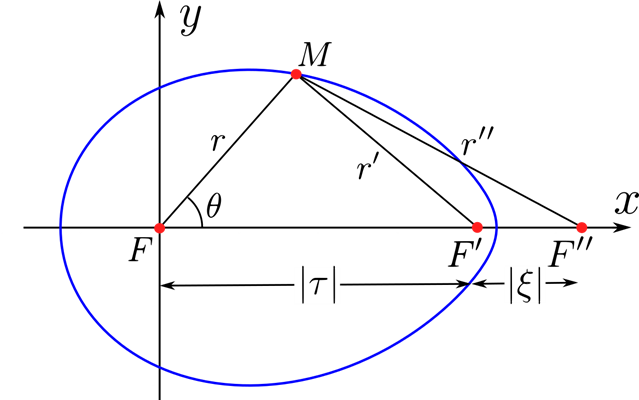
\includegraphics[width=0.55\linewidth]{images_low_resolution/cartesian_oval_v2.png}
	\caption{A Cartesian oval shown on the $xy$-coordinate system used in Section \ref{sec:Cartesian ovals}. The equation of the oval is $r+ar'=u$, with $a=0.6$ and $u=1.1$. The focal distances are $\tau=1$ and $\xi\simeq 0.36$.}	
	%\caption{A Cartesian oval with $\tau=1$, $a=0.7$ and $u=1.2$. The distances, angles, and other tags are also shown.}
	\label{fig:oval}
\end{figure}

\section{Characterization of the various orthogonal coordinates} %*Base coordenada, *Factores de escala, *elemento de línea
\label{sec:characterization}


%\section{Orthogonal systems of coordinates based on ovals} %2D (and 3D coordinates)
%\label{sec:orthogonal coordinates}
Consider the rectangular Cartesian coordinates $x,y$ in the $xy$-plane. Any two coordinates $q^1,q^2$, related to the rectangular ones by the equations $x=x(q^1,q^2)$ and $y=y(q^1,q^2)$, are said to be orthogonal if their metric coefficients,
\be
	g_{ij} = \partd{\mb{r}}{q^i} \cdot \partd{\mb{r}}{q^j}\,, \label{eq:def g_ij}
\ee
form a diagonal matrix, where $\mb{r}=x(q^1,q^2)\ihat+y(q^1,q^2)\jhat$ is the position vector of the point $(x,y)$ in the $xy$-plane and $\ihat,\jhat$ are the unitary Cartesian vectors. It is not difficult to see that the orthogonality condition for $q^1,q^2$ is 
\be
x_{,1}x_{,2}+y_{,1}y_{,2}=0\,, \label{eq:orthog. cond1}
\ee
where the subscripts indicate partial differentiation, $x_{,i}:=\partial x/\partial q^i$ for each $i=1,2$.

This condition is equivalent to say that the $q$-constant curves, called the coordinate curves, intersect each other at right angles, as it is shown in the appendix \ref{sec:appendix}. Hence, to construct a 2D system of coordinates, it is sufficient to have a pair of uniparametric families of curves $\mathscr{F}_1=\cub{\gamma_r}_{r\in\mathcal{I}}$ and $\mathscr{F}_2 = \cub{\sigma_s}_{s\in\mathcal{J}}$ so that if $\gamma\in\mathscr{F}_1$ and $\sigma\in\mathscr{F}_2$ then $\gamma$ and $\sigma$ meet at right angles. The parameters of these two families $r,s$ may be taken as the $q^i$-coordinates. Naturally, to any point in the $xy$-plane must pass one and only one member of each family.

If, in addition, these families $\mathscr{F}_1,\mathscr{F}_2$ can be seen as the level curves of two functions $f,g$, respectively, then $r=f(x,y)$ and $s=g(x,y)$ are the relations between Cartesian and $rs$-coordinates. Their inversion, $x=x(r,s), y=y(r,s)$, would allow to compute the metric coefficients in terms of $r$ and $s$. To construct \textit{oval} coordinates, one may consider that one, or both, of the coordinate curves are ovals. In the next sections, two special families of ovals are considered: confocal ovals and triconfocal ovals. With them, various orthogonal coordinates will be built.


%\section{Characterization of the various orthogonal coordinates} %*Base coordenada, *Factores de escala, *elemento de línea
%\label{sec:characterization}
Confocal and triconfocal ovals induced certain systems of coordinates in which the coordinate curves are one of these class of ovals. In this section we will characterize these coordinates in terms of their metric coefficients and their basis vectors. From the methods mentioned in \cite{moon1988field}, 3D coordinates will be constructed from the 2D coordinates by ``rotating'' or ``translating'' the coordinates. This process results in cylindrical- and rotational-like coordinates, respectively. %%CORRECCIÓN: Añadir referencias a los otros artículos de Moon y Spencer

Consider confocal ovals as $u$-constant curves and synecdolas as $v$-constant ones. The quantities $u$ and $v$ define a set of \textit{confocal oval 2D coordinates}, or simply \textit{oval coordinates}. The metric coefficients are described in terms of the functions $x(u,v)\equiv \X(u,v)$ and $y(u,v)\equiv\Y(u,v)$ as
\be
	 ds^2 = \rob{\X_u^2+\Y_u^2}(du^2 + \Y^2 dv^2)\,,
\ee
where the subscripts indicates partial differentiation. These function satisfy the relations
\be	
	\X_{u} = 
-\frac{\sqrt{\X^{2}+\Y^{2}}\,a \left(\tau -\X \right) -\X  \sqrt{(\X-\tau)^2 + \Y^2}}{2 a \left(\X^{2}+\Y^{2}-\X\tau\right)+ \left(a^{2}+1\right) \sqrt{\X^{2}+\Y^{2}} \sqrt{(\X-\tau)^2 + \Y^2} } \,, \label{eq:diff1}
\ee
\be	
	\Y_{u} = 
\frac{\Y \left(\sqrt{\X^{2}+\Y^{2}}\, a +\sqrt{(\X-\tau)^2 + \Y^2}\right)}{2 a \left(\X^{2}+\Y^{2}-\X\tau\right)+ \left(a^{2}+1\right) \sqrt{\X^{2}+\Y^{2}} \sqrt{(\X-\tau)^2 + \Y^2} } \,,\label{eq:diff2}
\ee
\be 
	\X_v = \Y\Y_u\,, \label{eq:diff3}
\ee
\be
	\Y_v = -\Y\X_u\,,  \label{eq:diff4}
\ee
which can be obtained by taking partial differentiation to the equations $u=\sqrt{x^2+y^2}+a\sqrt{(x-\tau)^2+y^2}$ and $v=\arcsinh(x/y)+a\,\arcsinh((x-\tau)/y)$, which define $u$ and $v$ in terms of $x$ and $y$. In addition, the basis vectors related to $u$ and $v$ are
\be
	\ehat_u = \frac{1}{\sqrt{\X_u^2 + \Y_u^2}}\rob{\X_u\ehat_x + \Y_u\ehat_y }\,,
\ee
\be
	\ehat_v = \frac{1}{\sqrt{\X_u^2 + \Y_u^2}}\rob{\Y_u\ehat_x-\X_u\ehat_y}\,.
\ee

Another system of coordinates may be derived from triconfocal ovals. The quantities $\alpha$ and $\beta$, defined in the previous section, are consider as a set of \textit{triconfocal oval 2D coordinates}, or \textit{triconfocal coordinates} for short. In this case, the metric coefficients are given by
\be
	ds^2 = g_{\alpha\alpha}\rob{d\alpha^2+\frac{(\alpha^2-1)(\alpha^2\xi-\tau-\xi)}{(1-\beta^2)(\beta^2\xi-\tau-\xi)} d\beta^2}\,,
\ee
with
\begin{multline}
	g_{\alpha\alpha} = \Big[2 \rob{-\alpha  \beta  \xi +\tau +\xi } \sqrt{\tau^{2} \rob{\beta^{2} \xi -\tau -\xi } \rob{\alpha^{2} \xi -\tau -\xi }}+ \big(2\rob{\alpha^{2} \beta^{2}+1} \xi \\
	 -\rob{\beta +\alpha }^{2} \rob{\xi +\tau }-4 \tau \big) \xi  \tau +2 \tau^{3}\Big] \frac{\beta +\alpha}{\rob{\alpha^{2}-1} \rob{\beta -\alpha }^{3} \rob{\alpha^{2} \xi -\tau -\xi }}\,.
\end{multline}
The basis vectors are ... In the case $\xi=0$, this coordinates get reduced to Pascal limaçon coordinates, whose metric coefficients are given by  %%CORRECCIÓN: Terminar de añadir o quitar la alusión a los vectores base en esta sección
\be
	ds^2=\frac{4(\alpha+\beta)\tau^2}{(\alpha-\beta)^3}\rob{\frac{1}{\alpha^2-1}d\alpha^2+\frac{1}{1-\beta^2}d\beta^2}\,.
\ee

Based on the two set of coordinates described before, one can easily obtain cylindrical-like coordinates. For this one just needs to introduce a $z$ coordinate in the orthogonal direction to the $xy$-plane in which the 2D coordinate curves live. Hence, one obtains \textit{confocal oval-cylinder coordinates} $u$, $v$ and $z$, and \textit{triconfocal oval-cylinder coordinates} $\alpha$, $\beta$ and $z$. Their line elements are respectively
\be
	ds^2 = \rob{\X_u^2+\Y_u^2}(du^2 + \Y^2 dv^2) + dz^2\,,
\ee
\be
	ds^2 = g_{\alpha\alpha}\rob{d\alpha^2+\frac{(\alpha^2-1)(\alpha^2\xi-\tau-\xi)}{(1-\beta^2)(\beta^2\xi-\tau-\xi)} d\beta^2} + dz^2\,.
\ee
It should be pointed out that the Laplace equation admits a separable solution for the triconfocal oval-cylinder coordinates, but not for the confocal ones.

Next, rotational coordinates can be obtained in the next way. Consider a point $(x(q^1,q^2),y(q^1,q^2),0)$ in some $xyz$-space related to coordinates $q^1$ and $q^2$. Rotate this point around either the $x$- or $y$-axis in a certain angle $\phi$. The set of points obtained by fixing one of the quantities $q^1$, $q^2$ and $\phi$ define a certain surface. The resulting classes of surfaces orthogonally intersect each other and define the coordinate surfaces of certain system of coordinates. Naturally, it only make sense to rotate the points around the symmetry axis of the coordinate 2D curves. For ovals, this coincides with the focal axis. 

Applying this to confocal ovals, one obtains the coordinates
\be
	\tilde{u} = \sqrt{x^2+y^2+z^2} + a \sqrt{x^2 + y^2 + (z-\tau)^2}\,, \label{eq:u(x;y;z)}
\ee
\be	
	\tilde{v} = \arcsinh\left( \frac{z}{\sqrt{x^2 + y^2}} \right) + a\, \arcsinh\left( \frac{z-\tau}{\sqrt{x^2 + y^2}} \right)\,, \label{eq:v(x;y;z)}
\ee
\be
	\phi = \text{atan2}(y,x)\,, \label{eq:phi(x;y;z)}
\ee
with inverse relations $x = \Y(\tilde{u},\tilde{v})\cos\phi$, $y = \Y(\tilde{u},\tilde{v})\sin\phi$ and $z = \X(\tilde{u},\tilde{v})$. The corresponding line element is
\be 
	ds^2 = \rob{\X_{\tilde{u}}^2+\Y_{\tilde{u}}^2}(d\tilde{u}^2 + \Y^2 d\tilde{v}^2) + \Y^2 d\phi^2\,. \label{eq:LE[ovoid]}
\ee
One can check that $\tilde{u}-$ and $\tilde{v}-$constant surfaces are surfaces of revolution of their respective coordinate curves around the symmetry axis. Since the surface of revolution of ovals are known as ovoids, this coordinates may be called as \textit{confocal ovoid 3D coordinates}, or simply as \textit{ovoid coordinates}. In the same spirit, the term \textit{synecdoloids} is coined to refer to the $\tilde{v}$-constant surfaces, in analogy to the one used for the surface of revolution of hyperbolas. The line element \ref{eq:LE[ovoid]} is the one that will be use in the next section to construct stationary spacetimes with ovoid symmetry.

Finally, for triconfocal oval coordinates one obtains
\be
	\tilde{\alpha} =  \frac{-\sqrt{z^2+x^2+y^2}\sqrt{(z-\tau)^2+x^2+y^2} + \tau \sqrt{(z-\tau-\xi)^2+x^2+y^2}}{(z-\tau)^2+x^2+y^2+\xi\tau}\,, \label{eq:alpha}
\ee
\be
	\tilde{\beta} = -\frac{\sqrt{z^2+x^2+y^2}\sqrt{(z-\tau)^2+x^2+y^2} + \tau \sqrt{(z-\tau-\xi)^2+x^2+y^2}}{(z-\tau)^2+x^2+y^2+\xi\tau}\,. \label{eq:beta}
\ee
\be
	\phi = \text{atan2}(y,x)\,, \label{eq:phi(x;y;z)}
\ee
with the inverse relations $x = \kappa(\tilde{\alpha},\tilde{\beta})\cos\phi$, $y = \kappa(\tilde{\alpha},\tilde{\beta})\sin\phi$ and $z = \eta(\tilde{\alpha},\tilde{\beta})$, where $\eta(\alpha,\beta)$ is taken to be the right hand side of the equation \ref{eq:xAB} and $\kappa(\alpha,\beta)$ is taken to be the square root of the right hand side of the equation \ref{eq:yAB}. The quantity $\phi$ takes values in the interval $[0,2\pi)$, and as in the previous section $\tilde{\alpha}\in\mathcal{D}_{\tilde{\alpha}}$ and $\tilde{\beta}\in\mathcal{D}_{\tilde{\beta}}$. The line element is
\be
	ds^2 = g_{{\tilde{\alpha}}{\tilde{\alpha}}}\rob{d{\tilde{\alpha}}^2+\frac{({\tilde{\alpha}}^2-1)({\tilde{\alpha}}^2\xi-\tau-\xi)}{(1-{\tilde{\beta}}^2)({\tilde{\beta}}^2\xi-\tau-\xi)} d{\tilde{\beta}}^2} + \kappa^2d\phi^2\,.
\ee
This coordinates may be called as \textit{triconfocal ovoid 3D coordinates}.

\begin{table}[hb]
	\centering
	\caption{Orthogonal coordinates. $\mathcal{D}_u$ is given by the equation \ref{eq:D_u} and $\mathcal{D}_\alpha$ and $\mathcal{D}_\beta$ are described in Section \ref{sec:triconfocal}. For the Pascal limaçon coordinates it was made $\alpha\equiv\mu$ and $\beta\equiv\nu$.}
	\begin{tabular}{lcccc}
	\hline
	System of coordinates & Coordinates & \multicolumn{3}{c}{Conditions} \\ \hline
	\textit{Confocal oval coordinates}	& $u,v$ & $u\in\mathcal{D}_u$ & $v\in\Re$& \\
	\textit{Confocal oval-cylinder coordinates} & $u,v,z$ & $u\in\mathcal{D}_u$& $v\in\Re$ & $z\in\Re$ \\
	\textit{Confocal ovoid coordinates} & $\tilde{u},\tilde{v},\phi$ & $\tilde{u}\in\mathcal{D}_{u}$ & $\tilde{v}\in\Re$ & $\phi\in[0,2\pi)$ \\
	\textit{Triconfocal oval coordinates} & $\alpha,\beta$ & $\alpha\in\mathcal{D}_\alpha$ & $\beta\in\mathcal{D}_\beta$ & \\
	\textit{Pascal limaçon coordinates} & $\mu,\nu$ & $\mu\in[-1,1]$& $\nu\in(-\infty,-1]$ \\
	\textit{Triconfocal oval-cylinder coordinates} & $\alpha,\beta,z$ & $\alpha\in\mathcal{D}_\alpha$& $\beta\in\mathcal{D}_\beta$& $z\in\Re$ \\
	\textit{Triconfocal ovoid coordinates} & $\tilde{\alpha},\tilde{\beta},\phi$ & $\tilde{\alpha}\in\mathcal{D}_\alpha$& $\tilde{\beta}\in\mathcal{D}_\beta$& $\phi\in[0,2\pi)$ \\ \hline
	\end{tabular}
	\label{tab:existence}
\end{table}

%% CORRECCIÓN: Añadir una mensión a la tabla, así como añadir imágenes de las curvas y superficies coordenadas. Discutir acerca de estas imágenes

% (Listo!) Oval coordinates (2D)
% (Listo!) Cylindrical ovoid coordinates (3D)
% (Listo!) (Rotational) ovoid coordinates (3D)

% (Listo!) Triconfocal oval coordinates (2D)
% (Listo!) Triconfocal cylindrical ovoid coordinates (3D)
% (Listo!) Triconfocal (Rotational) ovoid coordinates (3D)

\section{Ovoid spacetimes} %*Talk a little about the Krasinski method *Propose the metric ansatz for Conformally stationary (biconfocal) triconfocal spacetimes
\label{sec:ovoid spacetimes}
The symmetries in a spacetime are usually characterized by geometric invariants such as Killing vectors. These vector can be associated to a group of isometries isomorphic to a certain group such as $SO(2)$ or $SO(3)$. In this sense, it is natural to define an axially symmetric spacetime or a spherically symmetric spacetime as one in which there is a subgroup $G$ of the group of isometries\footnote{$\text{Iso}(M,\mc{G}):=\cub{\phi:M\to M\mid \phi^{*}\mc{G}=\mc{G}}$ endowed with the composition operation, where $M$ is the manifold, $\mc{G}$ is the metric tensor and $\phi^{*}$ is the pushforward of $\phi$.} which is isomorphic to $SO(2)$ or $SO(3)$, respectively. However, for other spacetimes such as ellipsoidal or ovoid spacetimes, there is not such a natural definition since there is not a group related to ellipsoids or ovoids. The best one can do is to propose a metric ansatz that encapsulates some desirable features. One of such may be that, for example, there exits some congruence of observers in which the induced metric over their orthogonal hypersurfaces resembles or be similar to the metric over ellipsoids or ovoids. Such proposal is the one of Krasiński \cite{Krasinski1978}, which construct an stationary oblate-ellipsoidal metric ansatz. Here, a stationary ovoid metric ansatz will be built based on the same procedure. %%CORRECCIÓN: Añadir referencias al libro de Sthefani-Kramer-...

In order to do that, consider a congruence of observers characterized by the four-velocity $w= U\partial_t + V \partial_\phi$. As the spacetime is consider to be stationary and axially symmetric, there exist two conmuting killing vector fields, which here are considered as $\partial_t$ and $\partial_\phi$. The projection of the metric tensor over the orthogonal hypersurfaces of $w$ is taken as
\be
	(g_{ab}+w_a w_b)dx^a \otimes dx^b = f^2(\X_u^2+\Y_u^2) du \otimes du + k^2\sqb{\Y^2(\X_u^2+\Y_u^2)dv\otimes dv + \Y^2 d\Phi\otimes d\Phi}\,,\label{eq:h_ab}
\ee
%\be
%	g_{ab}+u_au_b = f^2(\X_u^2+\Y_u^2)(\mb{d}\mbi{u})_a(\mb{d}\mbi{u})_b+k^2\sqb{\Y^2(\X_u^2+\Y_u^2)(\mb{d}\mbi{v})_a(\mb{d}\mbi{v})_b + \Y^2(\mb{d}\mbi{\phi})_a(\mb{d}\mbi{\phi})_b}\,,
%\ee
where $f$ and $k$ are functions of $u$ and $v$, and $d\Phi = d\phi-(V/U)dt$. From here one can deduce the most general form of a metric tensor that satisfies the equation \ref{eq:h_ab}, which is
\begin{align}
	\mathcal{G} = g_{00} dt\otimes dt &+ g_{03}(dt\otimes d\phi + d\phi \otimes dt) + A^2 d\phi \otimes d\phi + f^2(\X_u^2+\Y_u^2) du\otimes du\notag \\ 
	&+ k^2\Y^2(\X_u^2+\Y_u^2)dv\otimes dv\,.  \label{eq:G}
\end{align}

Over the 2-surfaces spanned by the vectors $\partial_v$ and $\partial_\phi$, the induced metric is conformal to that of an ovoid (see equation \ref{eq:LE[ovoid]}). To simplify the notation, the tilde emphasis in $u$ and $v$ has been omitted. Equation \ref{eq:h_ab} shows that there is a part of the induced metric that is conformal to the metric over confocal ovoids, with $k^2$ being the conformal factor. The same procedure describe before can be implemented to derive a triconfocal ovoid metric ansatz $\mathcal{G}'$. For simplicity, this article focus only on this confocal case. Now it is convenient to write the static case of the metric $\mathcal{G}$ because it will be useful later. This corresponds to the metric
\be
	\mathcal{G}_{static}= g_{00} dt\otimes dt + k^2\Y^2 d\phi \otimes d\phi + f^2(\X_u^2+\Y_u^2) du\otimes du\\ + k^2\Y^2(\X_u^2+\Y_u^2)dv\otimes dv\,. \label{eq:G_static}
\ee

It should be mention that by considering the equations \ref{eq:diff1} and \ref{eq:diff2} to write $\X_u$ and $\Y_u$ in terms of $\X=z$ and $\Y=\sqrt{x^2+y^2}$ and by fixing $a=0$ or $\tau=0$, $\mathcal{G}_{static}$ in spherical coordinates is reduced to
\be
\mathcal{G}_{spheric}= g_{00} dt\otimes dt + k^2r^2{\sin^2{\theta}}\, d\phi \otimes d\phi + f^2 dr\otimes dr\\ + k^2r^2 d\theta \otimes d\theta\,.
\ee
which is a suitable metric ansatz to describe static spherically symmetric spacetimes. Hence, the \textit{ovoid spacetimes} here described have the spherically symmetric spacetimes as a particular case. The condition $a=0$ or $\tau=0$ makes the $u$-constant surfaces in the ovoid coordinate system become concentric spheres to the origin with radius $r=u$ or $r=u/(1+a)$, respectively.

%%CORRECCIÓN: Revisar definiciones de dPhi, añadir g_00 y g_03

\section{Anisotropic fluid solutions to the Einstein field equations}
\label{sec:solutions}
The relevance to define spacetimes with new symmetries is that it opens the possibility to obtain new exact solutions to the Einstein field equations. If it is a vacuum solution, it can be interpreted as the solution for a black hole ore one part of it can be interpreted as the external solution for an object with ovoid symmetry. And, if it is a fluid solution, one would obtain a model for the gravitational field inside an object with ovoid symmetry. Both cases are very interesting and stimulating. Sadly, the Einstein field equations get too complicated. For this article, only a static anisotropic fluid solution is obtained.

Consider a static ovoid spacetime govern by the metric $\mathcal{G}_{static}$. A suitable stress-energy tensor for an static anisotropic fluid is
\be
	\mathcal{T} = T^{ab} \partial_a\otimes \partial_b = (\mu+P_1)w\otimes w+P_1\mathcal{G}_{static}^{-1} + (P_2-P_1) e_2\otimes e_2 + (P_3-P_1)e_3\otimes e_3\,,
\ee
where $w$ is the four-velocity of the fluid, $\mu$ is its mass-energy density, $P_i$ is its pressure in the direction of $e_i$ with $i=1,2,3$, $\{e_\mu\}=\{w,e_1,e_2,e_3\}$ is the orthonormal tetrad of the observer with four-velocity $w$, and $\mathcal{G}_{static}^{-1}$ is the inverse metric. Naturally, the quantities $\mu$ and $P_i$ are the ones measured by the comoving observer with the fluid. In the case $P_2=P_3=P_1$ one recovers the stress-energy tensor of a perfect fluid in its standard form. In natural units the Einstein field equations are
\be
	R_{ab} = 8\pi\rob{ T_{ab}-\frac{1}{2}T g_{ab}}\,, \label{eq:EFE}
\ee
where $T$ is the trace of $\mathcal{T}$ and $\mathcal{R}=R_{ab}\,dx^a\otimes dx^b$ is the Ricci tensor. 

A solution to this equations is given by
\be
	P_1 = \frac{1}{8\pi\Y^2(\X_u^2+\Y_u^2)^2}\rob{\mc{P}-A_u^2\Y^2(\X_u^2+\Y_u^2)e^{-2B}} \,,
\ee
\be
	P_2 = \frac{1}{8\pi\Y^2(\X_u^2+\Y_u^2)^2}\cub{\mc{L}-\sqb{(A_u+B_u)\Y_u-A_u^2\Y}(\X_u^2+\Y_u^2)\Y e^{-2B}}\,,
\ee
\be
	P_3 = \frac{1}{8\pi\Y^2(\X_u^2+\Y_u^2)^3}\cub{\mc{Q}+\sqb{A_u^2\Y^2(\X_u^2+\Y_u^2)-\mc{L}}(\X_u^2+\Y_u^2)e^{-2B}}\,,
\ee
\begin{align}
	\mu = \frac{1}{8\pi\Y^2(\X_u^2+\Y_u^2)^3}\big\{ -\mc{Q} &+ \big[2\Y^2A_{uu}+(B_u+5A_u)\Y\Y_u \notag \\
	&-A_u\Y^2(2B_u+3A_u)+\mc{P}\big](\X_u^2+\Y_u^2)^2e^{-2B} \big\}\,,
\end{align}
\be
	g_{00} = e^{2A}\,,
\ee
\be
	f = e^{2B}\,,
\ee
\be
	k = e^{2(c_1-A)}\,,	
\ee
where $A$ and $B$ are arbitrary functions of $u$, $c_1$ is a constant, and $\mathcal{P}$, $\mathcal{Q}$ and $\mathcal{L}$ are given by
\be
	\mathcal{P} = \Y_u\rob{\Y_{uv}\X_u-\X_{uv}\Y_u}(e^{2(A-c_1)}-e^{-2B})\,,
\ee
\begin{align}
	\mathcal{Q} =& 	\sqb{(\X_u^2-\Y_u^2)(\Y_{uv	}^2+\X_{uv}^2) + (\X_u \X_{uvv}+\Y_u \Y_{uvv})(\X_u^2+\Y_u^2) - 4\X_u \Y_u \X_{uv} \Y_{uv}}\notag\\
	&\times (e^{2(A-c_1)}-e^{-2B}) +(A_u+B_u)(\X_u^2+\Y_u^2)(\X_u \Y_{uv}-\Y_{u}\X_{uv})\Y e^{-2B} \,,
\end{align}
\be
	\mathcal{L} = \X_u\rob{\X_{uv}\X_u + \Y_{uv}\Y_u}(e^{-2B}-e^{2(A-c_1)})\,,
\ee

In order to check that this solutions satisfies the equation \ref{eq:EFE} it is convenient to use the relations shown in Section \ref{sec:appendix-XY} to simplify the expressions that involve derivatives of $\X$ and $\Y$. In this scenario, the weak and strong energy conditions can be satisfied if $\mu,P_i\geq 0$. In the limit when $x,y,z\gg \tau$ this inequalities take the approximate form 
\be
	uA_u^2-(A_u+B_u) \geq 0\,,
\ee
\be 
	1-e^{2(A+B-c_1)}-u^2A_u^2\geq 0\,,
\ee
\be
	2A_u-uA_uB_u+uA_{uu}-uA_u^2\geq 0\,.
\ee
These were obtained by expressing the derivatives of $\X$ and $\Y$ in terms of themselves (see the appendix \ref{sec:appendix-XY}) and taking the high order terms in $x$, $y$ and $z$. A solution to the exact or the approximate energy conditions is left for a future work.


%%%%%%%%%%%%%%%%%%%%%%%%%%%%%%%%%%%%%%%%%%%%%%%%%%%%%%%%%%
%%%%%%%%%%%%%%%%%%%%%%%%%%%%%%%%%%%%%%%%%%%%%%%%%%%%%%%%%%
\section{Conclusions}
\label{sec:conclusions}

%%%%%%%%%%%%%%%%%%%%%%%%%%%%%%%%%%%%%%%%%%%%%%%%%%%%%%%%%%
%%%%%%%%%%%%%%%%%%%%%%%%%%%%%%%%%%%%%%%%%%%%%%%%%%%%%%%%%%
\bibliographystyle{unsrt}
\bibliography{OC_Ref}



\section{Appendix}
\label{sec:appendix}

%\subsection{Existence condition for Cartesian ovals}
%The existence conditions of ovals may be simplified by introducing the set $\mathcal{D}_u$ given by
%\be
%	\mathcal{D}_u(a;\tau) := \begin{dcases}  
%		[\text{min}{(1,a)}|\tau|,\infty) &\text{if   }a>-1\,; \\	
%		[-|\tau|,|\tau|] &\text{if   }a=-1\,; \\
%		(-\infty,|\tau|] &\text{if   }a<-1\,.
%	\end{dcases} \label{eq:D_u}
%\ee


%\subsection{Orthogonality condition for coordinates $q_1,q_2$}
%Here, it is shown that any two coordinates $q_1,q_2$ are orthogonal if and only if their coordinate curves meet at right angles. To do so, consider the relations $q^i=q^i(x,y)$ and their gradient $\bnabla q^i$. Since $\bnabla q^i$ is orthogonal to the level curves of $q^i$ then the coordinate curves intersect at right angles if
%\be
%	\bnabla q^1 \cdot \bnabla q^2 = q^1_{x}q^2_{x}+q^1_{y}q^2_{y} = 0\,, \label{eq:orthog. cond2}
%\ee
%where the subscripts indicate partial differentiation, $q^i_x:=\partial q^i/\partial x$ for each $i=1,2$. By the chain rule one has that
%\be
%	\partd{q^i}{q^j} = q^i_{x}x_{,j}+ q^i_{y}y_{,j}\,,
%\ee
%for each $i=1,2$ and $j=1,2$. For $i\neq j$, $\partial q^i/\partial q^j=0$. Hence, in this case, one gets that $q^i_{x}=-q^i_{y}y_{,j}/x_{,j}$, which implies that $\bnabla q^1 \cdot \bnabla q^2 = q^1_{y}q^2_{y}(y_{,1}y_{,2} + x_{,1}x_{,2})/x_{,1}x_{,2}$, so that equation \ref{eq:orthog. cond1} implies equation \ref{eq:orthog. cond2}, and vice versa.

\subsection{The $s$-equation as an algebraic equation in some power of $s$}
\label{sec:appendix-s-equation}

\subsection{$r_1$ is the positive solution to the $s$-equation for $a=1/3$}
\label{sec:appendix-r1}

\subsection{Characterization of the second and third derivatives of the metric functions $\X$ and $\Y$}
\label{sec:appendix-XY}

%%%%%%%%%%%%%%%%%%%%%%%%%%%%%%%%%%%%%%%%%%%%%%%%%%%%%%%%%%

\end{document}
